\svnidlong
{$HeadURL: $}
{$LastChangedDate: $}
{$LastChangedRevision: $}
{$LastChangedBy: $}
\svnid{$Id: $}   


All models detailed in this Section are applicable to signatures states where 
 a photon, a W boson, a Z boson or a Higgs boson
 is radiated from the initial state partons instead of a gluon. 
The experimental signature is identified as \textit{V+\MET}.

\Todo{Add link to section describing EW bosons from a blob.}

Monojet searches are generally more sensitive
with respect to final states including bosons, due to the much
larger rates of signal events featuring quark or gluon radiation with
respect to radiation of bosons~\cite{Zhou:2013fla},
in combination with the low branching ratios if leptons from
boson decays are required in the final state.
The rates for the Higgs boson radiation is too low for these models
to be considered a viable benchmark~\cite{Carpenter:2013xra}.
However, the presence of photons,
leptons from W and Z decays,
and W or Z bosons decaying hadronically
allow backgrounds to be rejected more effectively,
making Z/gamma/W+\MET searches
still worth comparing with searches in the jet+\MET final state.

%\Todo{Additional motivations exist for this final state from SUSY searches.}
%TODO: Linda is writing sentence to make this stronger. 

% The three commonly chosen EFT benchmarks for Dirac dark matter that are
% kinematically distinct for what concerns the observables used in
% \MET+X searches~\footnote{[CD: we would need a plot here, or a reference to
% monojet section where this is shown]} and span a wide range of \MET spectrum in
% the boson+\MET searches are, in the notation of ~\cite{Goodman:2010ku},
% the D1 (scalar SM/WIMP interaction), D5 (vector-vector interaction) and D9
% (tensor interaction) operator.

In the case of a spin-1 mediator,
an example Feynman diagram for these processes can be constructed by taking
Fig.~\ref{fig:OP} and replacing the gluon with $\gamma,W$ or $Z$.
The interest for searches with W bosons in the final state
has been elevated by the increased cross section
for certain choices of couplings for a spin-1 mediator~\cite{Bai:2012xg}.
Run-1 searches have considered three sample cases for the product of
up and down quark couplings to the mediator, denoted as $\xi$:
\begin{itemize}
 \item[$\xi=0$:] Mediator couples to up-type or down-type quarks, but not both;
 \item[$\xi=1$:] Mediator couples to up-type and down-type quarks with same strength;
 \item[$\xi=-1$:] Mediator couples to up-type and down-type quarks with same strength, but opposite sign.
\end{itemize}
The $\xi=-1$ case leads to a large increase in the cross-section of the process,
and modifies the spectrum of missing transverse energy or
transverse mass used for the searches. The sensitivity of the W+\MET search for
this benchmark in this case surpasses that of the jet+\MET search.
However, as shown in Ref.~\cite{Bell:2015sza}, the cross-section increase is due
to the production of longitudinally polarized W bosons,
in violation of electroweak gauge symmetries. Unless further
particles are introduced (in a fashion similar
to the Higgs boson in the Standard Model), choosing a value of $\xi=-1$
for this simplified model will lead to a manifest violation of unitarity at LHC energies.
The simplified model with a vector mediator exchanged in the \schannel model
can still be considered as a benchmark for searches with a W boson if $\xi=1$.
We leave the study of further models with cross-section enhancements due
to different couplings to up and down quarks for studies beyond the early LHC searches
covered in this document.
An example of such model is the case of both DM and SM Higgs charged under a new $U(1)'$,
with a  small mass mixing between the SM Z-boson and the new \Zprime-boson.
This leads
to different effective DM couplings to $u_L$ and $d_L$, proportional to
their coupling to the Z boson, detailed in Appendix~\ref{app:EWSpecificModels_Appendix}.


%The scan in the parameters that characterize this simplified model for EW boson + \MET
%searches follow what is
%already detailed in Section~\ref{subsec:MonojetLikeModels}.


% CD: I tend to like this list so I'll leave it here in hope of recycling it
% \begin{itemize}
%  \item the mass of the DM particle ($m_{DM}$);
%  \item the mediator mass ($m_{Med}$);
%  \item the mediator width ($\Gamma_{Med}$);
%  \item the couplings between the DM and the mediator (\gdm),
%  and between the mediator and the initial state quarks ($g_{SM}$);
%  \item the chirality of the couplings between DM and mediator,
%  and between mediator and initial state quarks (vector-vector, axial-vector, axial-axial, vector-axial).
% \end{itemize}

As in the case of the jet+\MET models, the width does not have a significant
impact on the kinematic distributions relevant for those searches. An example
of the particle-level analysis acceptance using the
generator-level cuts from Ref.~\cite{Aad:2014tda}
for the photon+\MET analysis, but raising the photon $p_T$ cut
to 150~\gev is shown in Figure~\ref{fig:DMV_EW_gamma_acceptance},
comparing a width that is set to $\Gamma=M_{med}/3$ to the
minimal width (the ratio between the two widths
ranges from 1.05 to 1.5 with increasing mediator masses).

%% Redone as a table.
% mmed : minW
% 10  : 3.5
% 50 : 21.3
% 100 : 42.4
% 300 : 127.3
% 600 : 300.1
% 1000 : 503
% 3000 : 1512
% 6000 : 3024
\begin{table}[!h]
\begin{tabular}{| l |r r r r|}\hline
\multicolumn{5}{|c|}{Acceptance ratio for $\Gamma=\Gamma_{\rm min}$ vs
$\Gamma=\mMed/3$} \\ \hline 
\multicolumn{1}{|c|}{ } & \multicolumn{4}{c|}{\mdm/GeV}\\
\hline 
{\mMed/GeV}      & 10     & 50    & 200   & 400  \\ \hline
50   & 0.96   & 0.99  &       & 0.95 \\  
100  & 0.97   &       &       &      \\
300  & 1.00   & 1.02  &       &      \\
600  &        &       & 0.96  &      \\
1000 & 1.01   & 1.02  & 1.03  &      \\
3000 & 1.02   & 1.03  &       & 1.01 \\
\hline
\end{tabular}
    \caption{Analysis acceptance for the photon+\MET analysis when varying the mediator width, in the
    case of a vector mediator exchanged in the $s-$channel}%This plot will come from Marie-Helene
    \label{fig:DMV_EW_gamma_acceptance}
\end{table}

%% \begin{figure}
%%     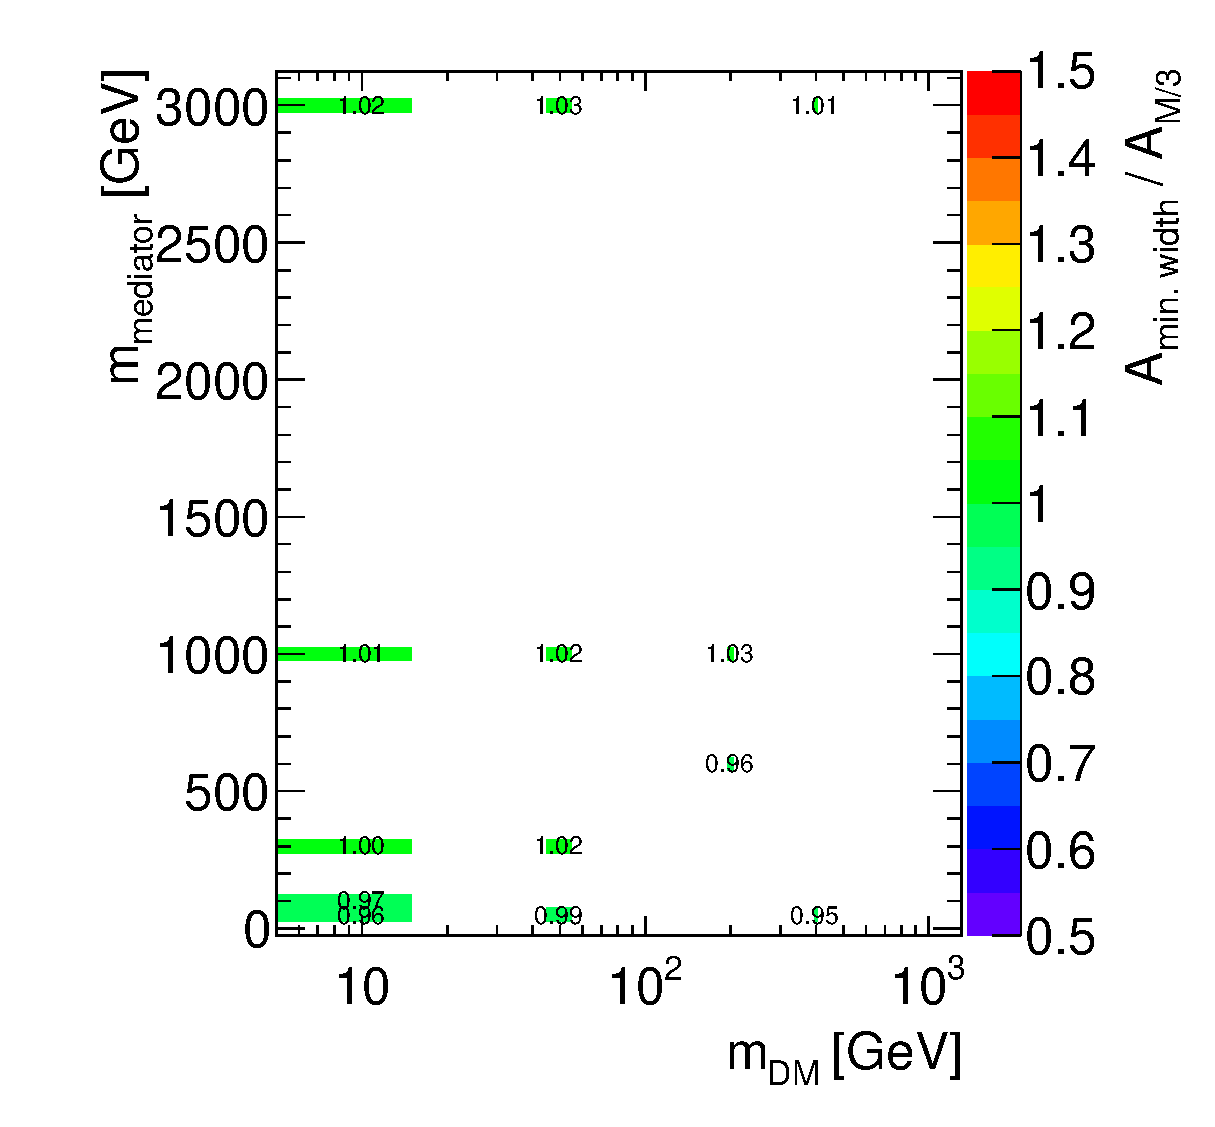
\includegraphics[width=0.7\textwidth]{figures/EW/acceptance_minwidth_vs_mo3_gamma}
%%     \caption{Analysis acceptance for the photon+\MET analysis when varying the mediator width, in the
%%     case of a vector mediator exchanged in the $s-$channel}%This plot will come from Marie-Helene
%%     \label{fig:DMV_EW_gamma_acceptance}
%% \end{figure}

Examples of relevant kinematic distributions for selected benchmark points are
shown in Fig.~\ref{fig:DMV_EW_kinematics_SVMed}. 
leading-order cross-sections for the chosen 
benchmark points are shown in Appendix~\ref{app:EWSpecificModels_Appendix}.

\begin{figure}[h!]
\centering  
\subfloat[Missing transverse momentum distribution for the photon+\MET final state, for 
different mediator mass choices, for \mdm=10~\gev.\label{fig:DMV_EW_gamma_MET_SVMed}]{%
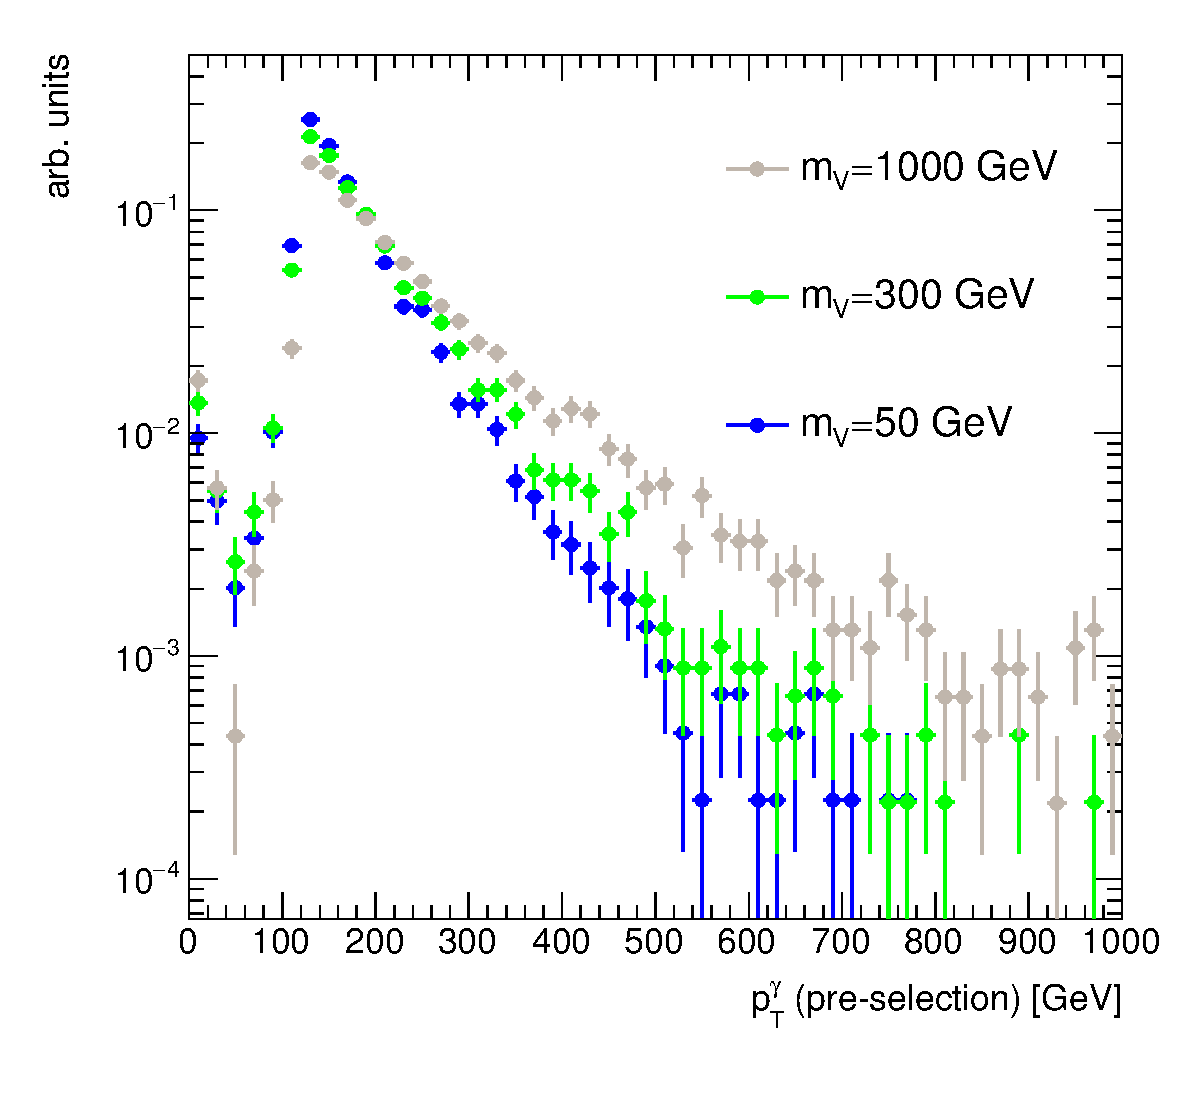
\includegraphics[width=0.45\textwidth]{figures/EW/ptGamma_filter120GeV_dmV_dm10GeV}
}%TODO: add this + equivalent plot of \MET to appendix
\hfill
\subfloat[Leading photon transverse momentum distribution for the photon+\MET final state, 
for different DM mass choices, with \mMed=1~\tev.\label{fig:DMV_EW_gamma_pT_SVMed}]{%
		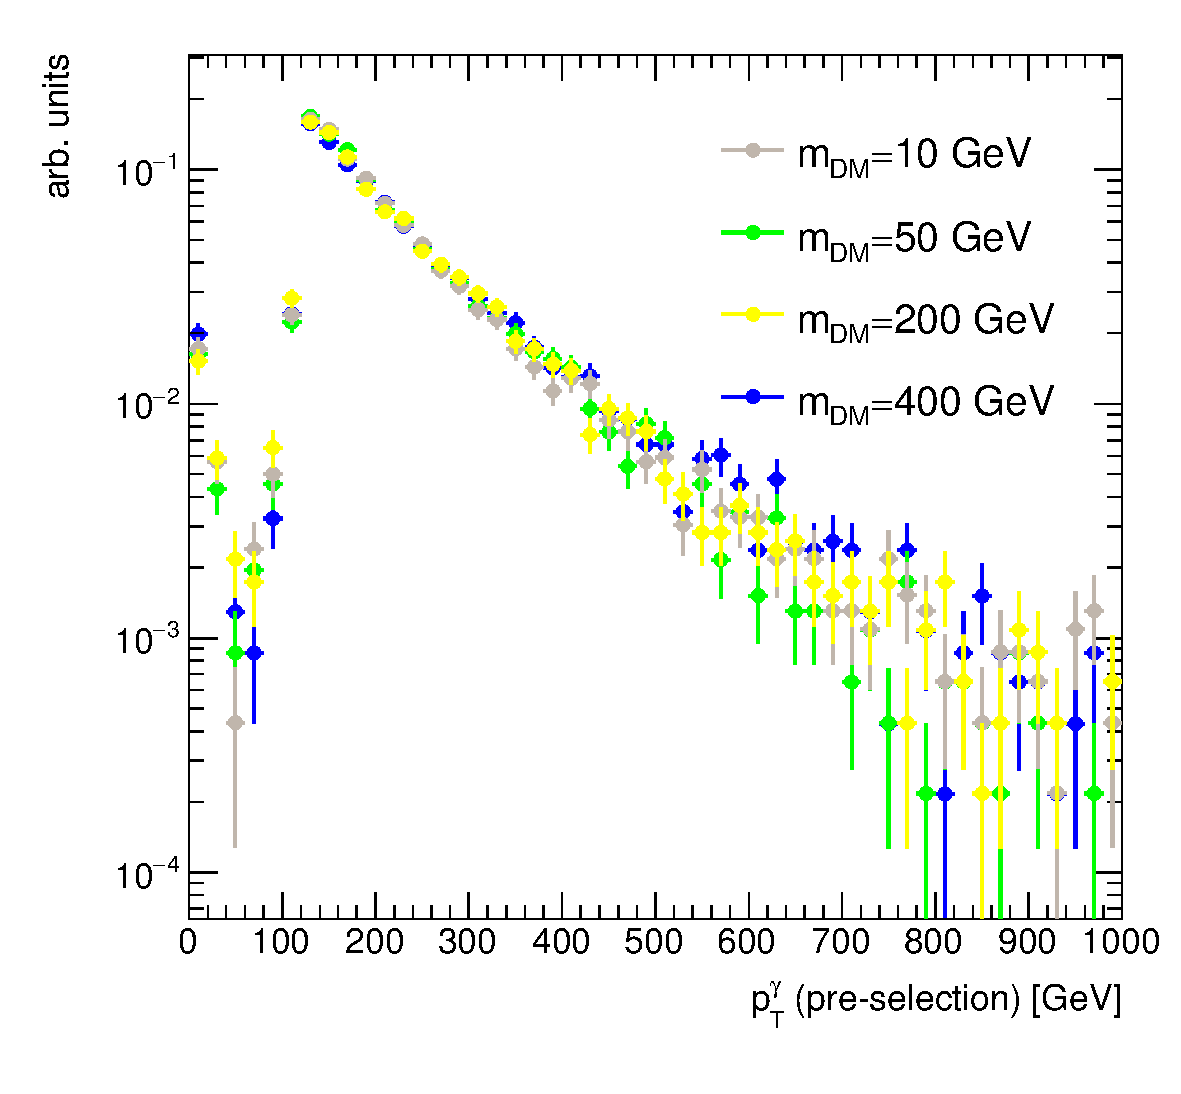
\includegraphics[width=0.45\textwidth]{figures/EW/ptGamma_filter120GeV_dmV_mV1000GeV}
}%TODO: add equivalent plot of \MET to appendix
\hfill
\subfloat[Missing transverse momentum distribution for the leptonic Z+\MET final state, 
for different mediator mass choices, for \mdm=15~\gev\label{fig:DMV_EW_Z_MET_SVMed}]{%
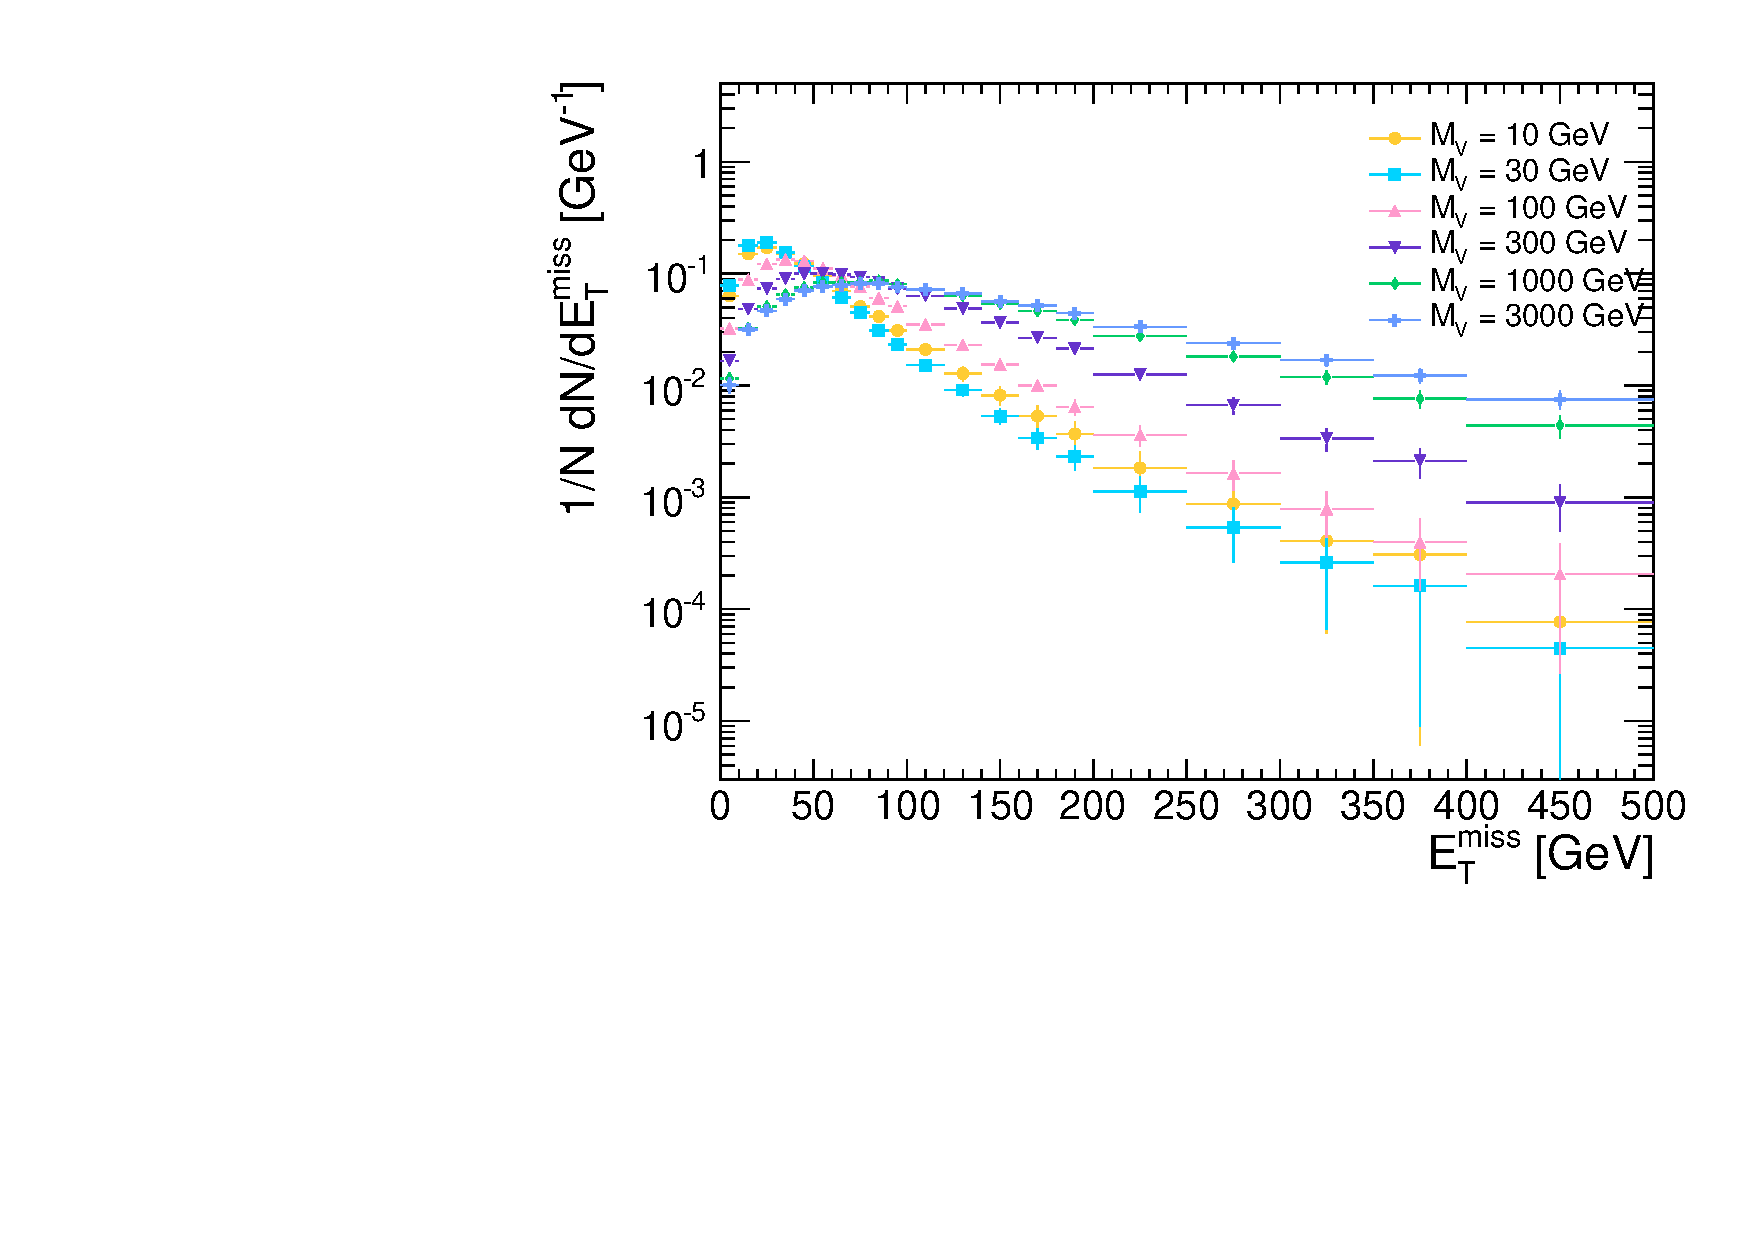
\includegraphics[width=0.45\textwidth]{figures/EW/pt_vv_Mx15}
}    
\hfill
\subfloat[Missing transverse momentum distribution for the hadronic W+\MET final state.\label{fig:DMV_EW_Whad_MET_SVMed}]{%
	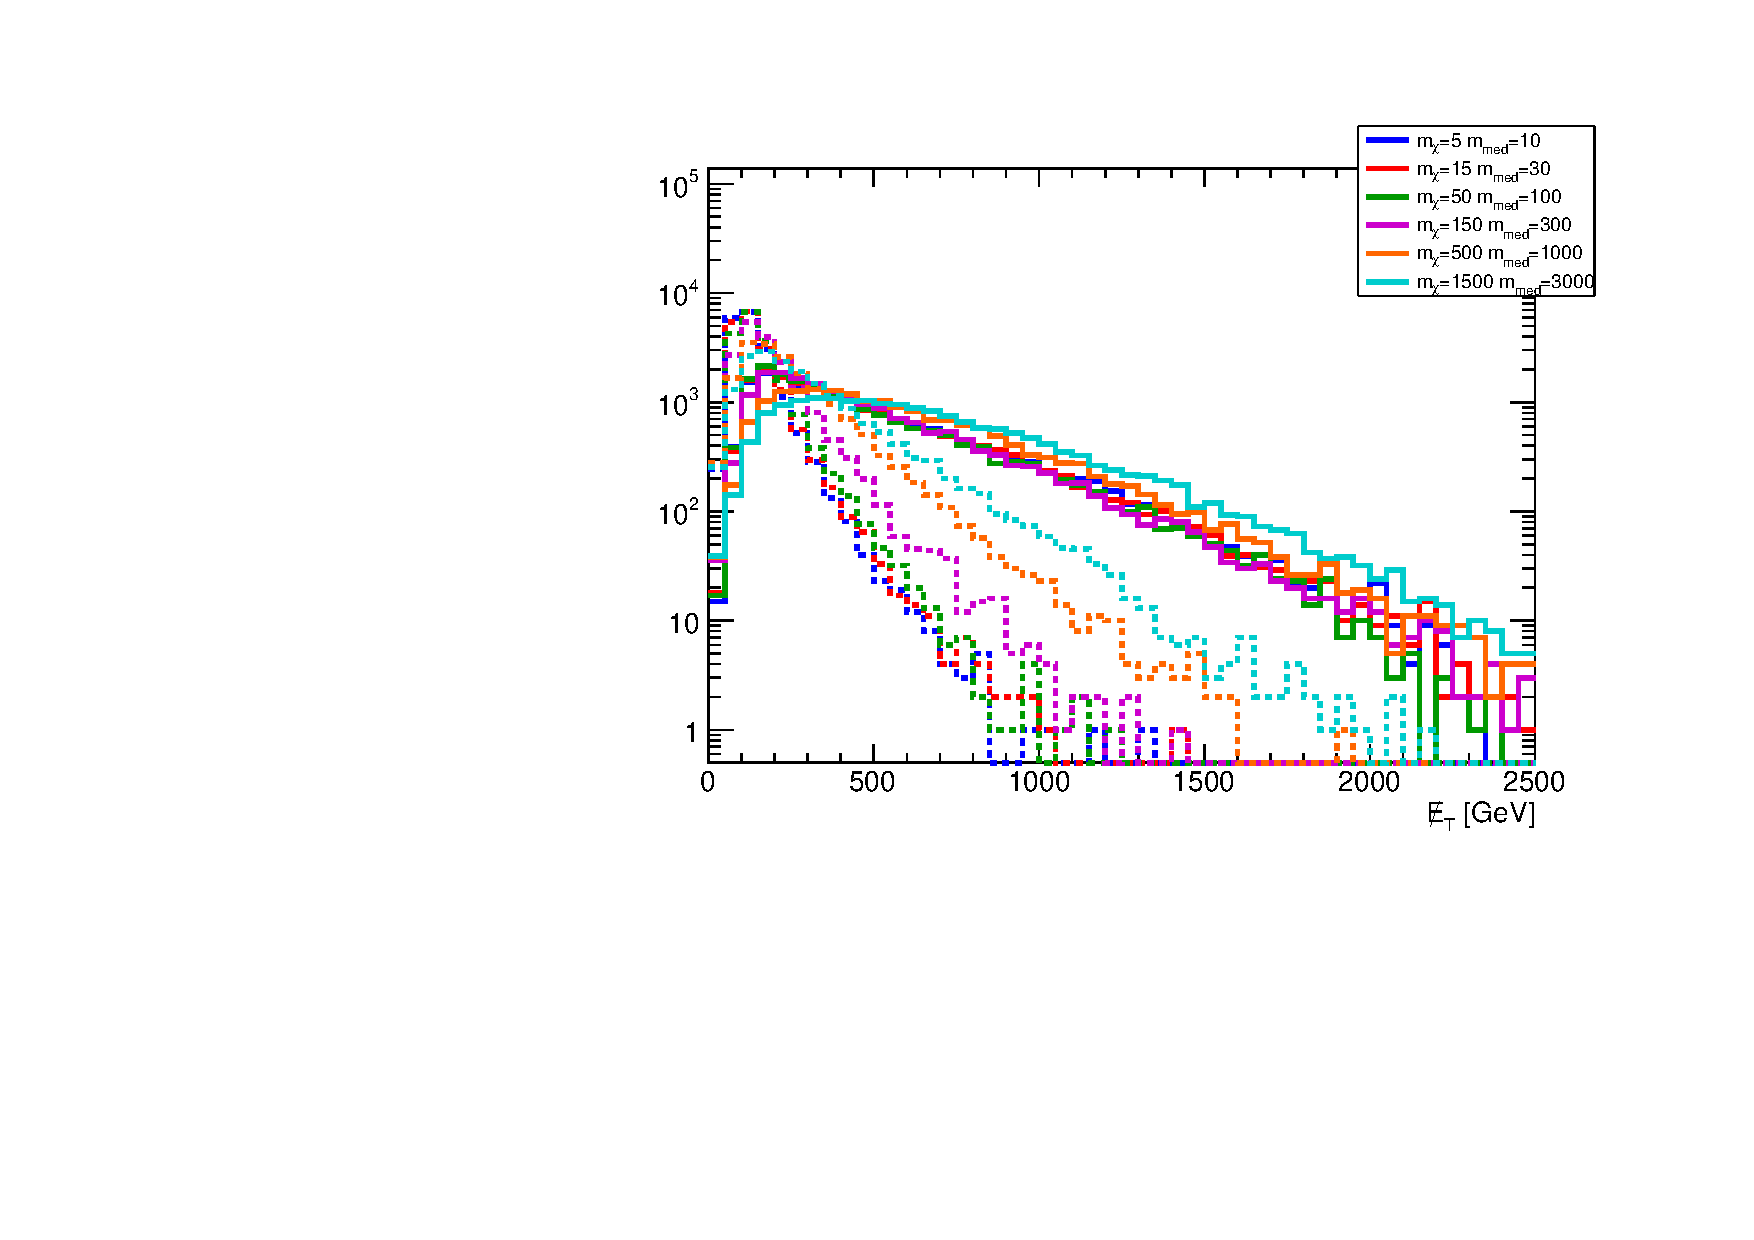
\includegraphics[width=0.5\textwidth]{figures/EW/monoWhad_Destructive/metPt}
}    
\caption{Kinematic distributions relevant for searches with W, Z and photons in the final state, 
for the simplified model
       with a vector mediator exchanged in the $s-$channel.}
\label{fig:DMV_EW_kinematics_SVMed}
\end{figure}
